\documentclass[11pt, twoside]{article}

\usepackage{graphicx}
\usepackage{amsmath}
\usepackage{amssymb}
\usepackage{verbatim} 
\usepackage{subfigure}
\usepackage{amsfonts}
%\usepackage{tikz}



\RequirePackage[usenames,dvipsnames]{color}
\RequirePackage{fancyhdr}
\RequirePackage{graphicx}

% to include C++ code:
\usepackage{listings}
\usepackage{xcolor}
\lstset { %
	language=C++,
	backgroundcolor=\color{black!5}, % set backgroundcolor
	basicstyle=\footnotesize,% basic font setting
}

%------------------- settings margini ----
\setlength{\oddsidemargin}{-15pt}
\setlength{\evensidemargin}{-15pt}
\setlength{\marginparwidth}{0pt}
\setlength{\textwidth}{500pt}
\setlength{\topmargin}{-40pt}
\setlength{\textheight}{650pt}

\newcommand{\cambiaFont}[2]{{\fontencoding{T1}\fontfamily{#1}%
		\selectfont#2}}

%-------- pacchetti base------------------
\usepackage[english]{babel}
\usepackage{euscript}
\usepackage[utf8]{inputenc}
%------ per i diagrammi commutativi: 
\usepackage{pictexwd,dcpic}
\usepackage[all]{xy}

%---- fancyheader and footer 
%\fancyhead{} % clear all fields
%\fancyhead[LE]{\thepage~~~~\textrm{asdf}~~\textit{asdffda}}
%\fancyhead[RO]{ {\sf Ricerca di Crittografia}, ~~~~\thepage}
\fancyfoot{}
\fancyfoot[RO]{ {\small  MPHYG002: Research Computing with C++, ~\thepage}}
\fancyfoot[LE]{ {\small \thepage,~ Coursework 2 }}
\renewcommand{\headrulewidth}{0.0pt}



\begin{document}

% %--------- pagenumbering ------------
\setcounter{page}{1}
\pagestyle{fancy} 
% %----------------------------------------



% ----  TITLE DATE ---- 
~\vspace{-2cm} 
\begin{center}  	
	
	\hrule
	
	\vspace{0.5cm} 
	\color{Black} MPHYG002: Research Computing with C++ \color{Black}
	\vspace{0.5cm} \\
	\cambiaFont{ppl}{ \color{MidnightBlue} $\bullet$ \color{MidnightBlue} ~{\Large Coursework 2 - Conway's Game of Life } ~ \color{MidnightBlue}$\bullet$\color{black}} 
	\vspace{0.3cm} \\
	Sebastiano Ferraris  ~ SN: 14108168 ~  s.ferraris@ucl.ac.uk ~ \today 
	\vspace{0.5cm} 
	\hrule
	
\end{center}

\vspace{0.1in}


%--- autore



%------------ indice eventuale:
 %\tableofcontents
%____________________________


\begin{center}
	\color{MidnightBlue} {\Large Part 1: Introducing the Game }\color{Black} 
\end{center}


\begin{center}
	\color{MidnightBlue} {\Large Part 1: Serial Solution }\color{Black} 
\end{center}


%\begin{figure}[htbp]
%	\centering
%	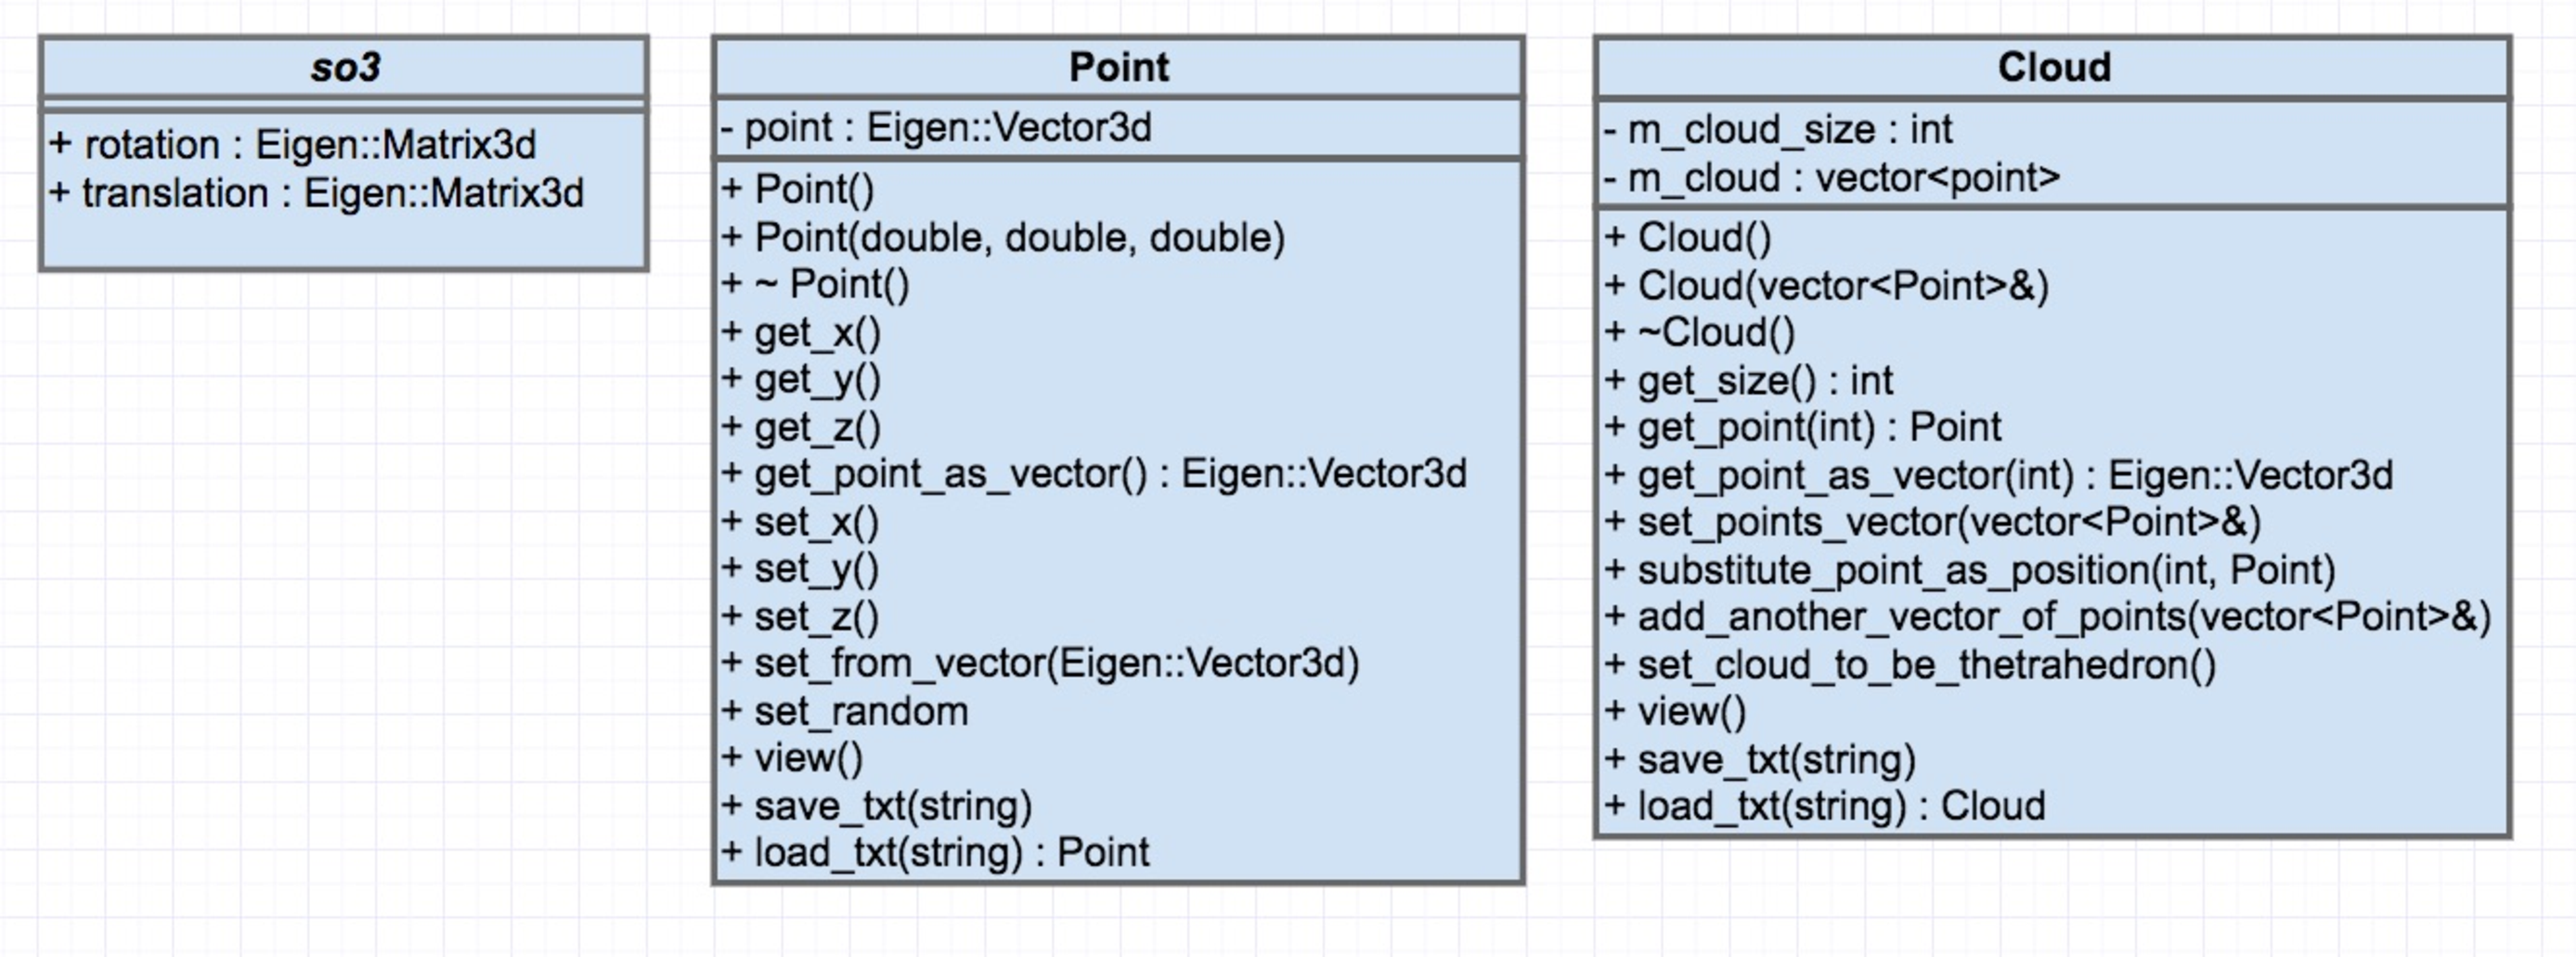
\includegraphics[scale=0.35]{figures/uml_diag.pdf}
%	\caption{UML diagram with the choice of the classes proposed for the implementation of the AHB algorithm.}
%	\label{fig:uml_diagram_classes}
%\end{figure}

\noindent
%\color{MidnightBlue} {\large  Exercise 2} \color{Black} \\
%\color{MidnightBlue}{\bf (a) }\color{Black} 
%Using the proposed framework, I implemented the AHB algorithm \cite{ahb_algo} in a simple folder structure under \emph{Code/registration\textunderscore3d\textunderscore point\textunderscore sets} divided into \emph{include}, \emph{source} and \emph{utils\textunderscore python}.
%\emph{Include} and \emph{source} contains respectively the header files and the source code. There are two .cc files with a main, that produces the actual applications: \emph{see\textunderscore methods.cc} and \emph{algo\textunderscore AHB.cc}. These can be called from the terminal under the path \emph{RCCPP-build/bin} in the build folder of the suggested framework. I choose an object oriented pattern, where one C++ structure, called \emph{so3}, and two classes, called \emph{Point} and \emph{Cloud}, are proposed. \\



\begin{center}
	\color{MidnightBlue} {\Large Part 2: Remote computation }\color{Black} 
\end{center}


qsub command here!


\begin{center}
	\color{MidnightBlue} {\Large Part 3: Shared memory parallelism }\color{Black} 
\end{center}



\begin{center}
	\color{MidnightBlue} {\Large Part 4: Distributed memory parallelism }\color{Black} 
\end{center}



\begin{center}
	\color{MidnightBlue} {\Large Part 5: Accelerated Solution }\color{Black} 
\end{center}

\begin{center}
	\color{MidnightBlue} {\Large Extra: between life and dead - a fuzzy game of life }\color{Black} 
\end{center}

\newpage
\begin{thebibliography}{2}
	
	\bibitem{ahb_algo}
	Arun, K. Somani, Thomas S. Huang, and Steven D. Blostein. "Least-squares fitting of two 3-D point sets." IEEE Transactions on pattern analysis and machine intelligence 5 (1987): 698-700.
	
	\bibitem{bmk_algo}
	Besl, Paul J., and Neil D. McKay. "Method for registration of 3-D shapes." Robotics-DL tentative. International Society for Optics and Photonics, 1992.
	
	\bibitem{cho_algo}
	Cho, Youngsang, et al. "A multi-resolution scheme for distortion-minimizing mapping between human subcortical structures based on geodesic construction on Riemannian manifolds." Neuroimage 57.4 (2011): 1376-1392.	
\end{thebibliography}
\end{document}





